\documentclass[11pt,a4paper]{article}
\usepackage[a4paper,margin=30mm]{geometry}
\usepackage[T1]{fontenc}
\usepackage{lmodern}
\usepackage{microtype}
\usepackage{booktabs,tabularx,longtable,array}
\usepackage{enumitem}
\usepackage{titlesec}
\usepackage{tikz}
\usetikzlibrary{arrows.meta,positioning,shapes.geometric,calc}
\usepackage{float}
\usepackage{xcolor}
\usepackage[colorlinks=true,linkcolor=blue,urlcolor=magenta]{hyperref}
\usepackage{caption}

% SRS template look: sans-serif bold headings, one chapter-like section per page.
\titleformat{\section}{\normalfont\sffamily\huge\bfseries}{\thesection}{0.6em}{}
\titleformat{\subsection}{\normalfont\sffamily\Large\bfseries}{\thesubsection}{0.6em}{}
\titleformat{\subsubsection}{\normalfont\sffamily\large\bfseries}{\thesubsubsection}{0.6em}{}
\titlespacing*{\section}{0pt}{30pt}{20pt}
\newcommand{\newsection}[1]{\clearpage\section{#1}}
\setlist{itemsep=1pt,topsep=3pt}
\renewcommand{\arraystretch}{1.3}
\newcommand{\rupee}{Rs.\,}

\tikzset{
  box/.style={draw,rounded corners=2pt,fill=blue!6,align=center,font=\small,inner sep=4pt},
  ext/.style={draw,fill=black!6,align=center,font=\small,inner sep=4pt},
  uc/.style={draw,ellipse,fill=yellow!10,align=center,font=\footnotesize,inner sep=1pt,minimum width=42mm,minimum height=6mm},
  ent/.style={draw,fill=orange!8,font=\footnotesize\bfseries,inner sep=4pt},
  proc/.style={draw,circle,fill=blue!6,align=center,font=\footnotesize,minimum size=19mm},
  store/.style={draw,align=center,font=\footnotesize,inner sep=3pt},
  state/.style={draw,rounded corners=3pt,fill=blue!6,font=\footnotesize,minimum width=19mm,minimum height=6.5mm},
  arr/.style={-{Stealth[length=2.2mm]},thin},
  lbl/.style={font=\scriptsize,fill=white,inner sep=1pt,align=center},
}

% Requirement table: ID | Requirement | Priority
\newenvironment{reqtable}{\par\noindent\tabularx{\linewidth}{@{}l X c@{}}\toprule
\textbf{ID} & \textbf{Requirement} & \textbf{Priority}\\\midrule}{\bottomrule\endtabularx\par\medskip}

\begin{document}

% ---------------- Title page (template layout) ----------------
\begin{titlepage}
  \vspace*{10mm}
  \noindent\rule{\linewidth}{4pt}\par
  \vspace{18mm}
  \begin{flushright}\bfseries
    {\Huge SOFTWARE REQUIREMENTS\\[4pt] SPECIFICATION\par}
    \vspace{14mm}
    {\Huge for\par}
    \vspace{14mm}
    {\Huge SV CAR CUSTOMS\par}
    \vspace{10mm}
    {\large Version 1.1 (final)\par}
    \vspace{18mm}
    {\large Prepared by : 1. Vishu Verma (1024170242)\\
     2. Raghu Verma (1024170241)\\
     3. Pratham Sharma (1024170229)\\
     4. Tarush Mohindru (1024170231)\par}
    \vspace{14mm}
    {\large Submitted to : Ms.\ Anushka\\
     UCS503 Software Engineering\par}
    \vspace{14mm}
    {\large November 26, 2026\par}
  \end{flushright}
\end{titlepage}

\tableofcontents
\clearpage

\section*{Revision History}
\begin{tabularx}{\linewidth}{@{}l l X@{}}
\toprule
\textbf{Version} & \textbf{Date} & \textbf{Changes} \\
\midrule
1.0 & 15 Oct 2026 & First version, submitted for the mid-semester evaluation. \\
1.1 & 26 Nov 2026 & Corrected to match the delivered system: customer login uses an
email OTP (SMS is used only for order updates); ``My Garage'' moved from future work to
implemented (FR-SRC-05); promo codes (FR-CHK-07) and guest-order linking (FR-ACC-06)
added; monitoring tools updated; requirement status column added in Section~3.3. \\
\bottomrule
\end{tabularx}

% =====================================================================
\newsection{Introduction}
\subsection{Purpose}
This document specifies the software requirements for \textbf{SV Car Customs}
(\url{https://www.svcarcustoms.in}), a web-based e-commerce platform that sells
aftermarket car accessories (body kits, spoilers, diffusers, exhausts, lighting,
paddle shifters, steering wheels and interior parts) from Delhi to customers across
India. It describes what the system must do, the quality levels it must meet, and the
constraints it works under. It is the agreed reference for design, implementation,
testing and future changes.

\subsection{Intended Audience and Reading Suggestions}
\begin{itemize}
  \item \textbf{Course instructor and evaluators} -- read Sections 1--2 for scope, then
        Section 3 for features and their delivery status.
  \item \textbf{Developers} (project team) -- Sections 3--5 give the testable
        requirements and interfaces.
  \item \textbf{Store owner / business stakeholder} -- Sections 1, 2 and 3 describe what
        the shop and the admin panel offer.
  \item \textbf{Testers} -- every requirement has an ID (e.g.\ FR-CAT-01) that test cases
        trace back to.
\end{itemize}

\subsection{Project Scope}
SV Car Customs previously sold through a hosted no-code storefront that gave little
control over search visibility, checkout, payments and product data. This project
replaces it with a custom-built platform that has two parts:
\begin{enumerate}
  \item a \textbf{customer storefront} where shoppers browse the catalogue by car model
        and part type, check vehicle fitment, add items to a cart, pay online (prepaid,
        or Cash on Delivery with a small advance) and track their orders; and
  \item an \textbf{admin panel} where the store owner manages products, categories,
        orders, promo codes, store settings, home-page content, leads and analytics.
\end{enumerate}
\textbf{In scope:} catalogue and search, vehicle fitment, cart, email-OTP login and guest
checkout, payment-gateway integration, order lifecycle and tracking, transactional
email and SMS, admin panel, SEO (sitemap, structured data, Google Merchant Center
feed), analytics and monitoring.\\
\textbf{Out of scope (v1.x):} native mobile apps, a marketplace for other sellers,
automated courier booking, multi-language UI, loyalty points and customer reviews.

\subsection{Objectives}
\begin{enumerate}
  \item Let a customer find a part that fits their car and complete a purchase in a
        few steps on a mobile phone.
  \item Give the owner full control of catalogue, prices, orders and settings without
        developer help.
  \item Rank on Google Search and Google Shopping for the store's products.
  \item Accept payments securely and never lose an order, even if a payment callback
        fails.
  \item Keep pages fast for Indian users (target under 2.5\,s Largest Contentful Paint
        on 4G).
\end{enumerate}

\subsection{Definitions, Acronyms and Abbreviations}
\begin{tabularx}{\linewidth}{@{}l X@{}}
\toprule
\textbf{Term} & \textbf{Meaning} \\
\midrule
PDP & Product Detail Page \\
SKU & Stock Keeping Unit -- one sellable variant of a product (e.g.\ colour) \\
Fitment & Mapping of a product to the car makes/models it fits \\
My Garage & The shopper's saved car, used to filter products that fit it \\
COD & Cash on Delivery \\
OTP & One-Time Password, sent to the customer's email \\
ISR & Incremental Static Regeneration -- cached pages refreshed on change \\
GST & Goods and Services Tax (India) \\
PayU & Payment gateway used for online payments \\
Admin & Store owner or staff with access to the admin panel \\
\bottomrule
\end{tabularx}

% =====================================================================
\newsection{Overall Description}
\subsection{Product Perspective}
SV Car Customs is a new, self-contained system that replaces a hosted third-party
store. It is built as a \textbf{monorepo} with a web front end and a separate REST API
that share typed request/response contracts, and it relies on several external
services (see Section~\ref{sec:design}).

\subsection{Stakeholders}
\begin{tabularx}{\linewidth}{@{}l X@{}}
\toprule
\textbf{Stakeholder} & \textbf{Interest / Role} \\
\midrule
Store owner (business) & Sells products, wants more orders, low running cost, full control of data. \\
Admin staff & Daily catalogue updates, order processing, COD collection. \\
Customers & Car owners and enthusiasts across India who want correct-fit parts and safe payment. \\
Guest visitors & Browse and buy without creating an account. \\
Development team & Vishu Verma, Raghu Verma, Pratham Sharma, Tarush Mohindru -- design, build, test, deploy. \\
Course instructor & Reviews requirements, design and progress. \\
Third-party providers & PayU, Resend, MSG91, Supabase, Vercel, Fly.io, Inngest, Google. \\
\bottomrule
\end{tabularx}

\subsection{User Classes and Characteristics}
\begin{itemize}
  \item \textbf{Guest} -- not logged in; can browse, search, use the cart and place an
        order with email, phone and address. Mostly on mobile; low to medium technical
        skill.
  \item \textbf{Registered customer} -- logs in with an email OTP (or a password they
        set); can view order history and saved addresses and track orders.
  \item \textbf{Admin} -- the store owner or staff; logs in to the admin panel with email
        and password; manages all store data. Uses both desktop and mobile.
  \item \textbf{System / automated actors} -- payment-gateway webhooks, background jobs
        and search-engine crawlers.
\end{itemize}

\subsection{Product Functions}
At a high level the system shall:
\begin{enumerate}
  \item Show a catalogue of products grouped by categories (car models and part types),
        with images, prices, variants and fitment.
  \item Let users search and filter products, including by their car (``My Garage'').
  \item Manage a cart and a checkout with address, pincode check, promo code and price
        breakdown (subtotal, discount, shipping, GST).
  \item Take payment through PayU as prepaid or COD-with-advance.
  \item Create orders, track their status and notify customers by email and SMS.
  \item Provide an admin panel for products, categories, orders, promo codes, settings,
        home page, leads, subscribers, analytics and an audit log.
  \item Publish SEO data: sitemap, robots rules, structured data and a Google Merchant
        Center product feed.
\end{enumerate}

\subsection{Operating Environment}
\begin{itemize}
  \item \textbf{Client:} any modern browser (Chrome, Safari, Firefox, Edge -- last two
        versions) on Android, iOS, Windows and macOS; responsive from 360\,px width.
  \item \textbf{Front end:} Next.js 16 (App Router, React 19, TypeScript) hosted on Vercel.
  \item \textbf{Back end:} Node.js 20 REST API built with Hono and Drizzle ORM, deployed
        as a Docker container on Fly.io (Mumbai region).
  \item \textbf{Database and files:} PostgreSQL and object storage on Supabase; Upstash
        Redis for cache and rate limits.
  \item \textbf{Background jobs:} Inngest (payment reconciliation, post-payment
        notifications, unpaid-order alerts).
  \item \textbf{Monitoring:} Sentry (errors), structured logs, first-party analytics and
        Google Search Console.
\end{itemize}

\subsection{Design and Implementation Constraints}
\begin{itemize}
  \item Payments must go through an RBI-compliant gateway (PayU); the system must never
        store card or bank details.
  \item Prices are shown inclusive of GST; GST rate and shipping rules must be
        configurable by the admin, not hard-coded.
  \item The team has four members and one semester; free or low-cost hosting tiers must
        be used.
  \item The code must be in TypeScript, kept in one Git repository, with automated tests
        (Vitest) run in CI before every release.
  \item Product claims (material, fitment, origin) must come from real product data, not
        be invented, to meet consumer-protection and Google Merchant Center policies.
\end{itemize}

\subsection{User Documentation}
The repository README gives setup and deployment steps; an admin guide covers adding a
product, processing an order and collecting COD. Customer help is given through the
FAQ, Shipping, Refund, Privacy and Terms pages.

\subsection{Assumptions and Dependencies}
\begin{itemize}
  \item Third-party services (PayU, Resend, MSG91, Supabase, Vercel, Fly.io, Inngest)
        remain available and within their plan limits.
  \item The owner supplies correct product data, prices and photos.
  \item Shipping is arranged manually by the owner through a courier; the system records
        shipment status but does not book couriers.
  \item Customers have a valid email address for login and an Indian mobile number for
        delivery and order updates.
\end{itemize}

\subsection{Design}\label{sec:design}
This section gives the main design diagrams: system context
(Figure~\ref{fig:ctx}), use cases (Figure~\ref{fig:uc}), data model
(Figure~\ref{fig:er}), data flow (Figure~\ref{fig:dfd}) and order life cycle
(Figure~\ref{fig:state}).

\subsubsection{System Context}
\begin{figure}[H]\centering
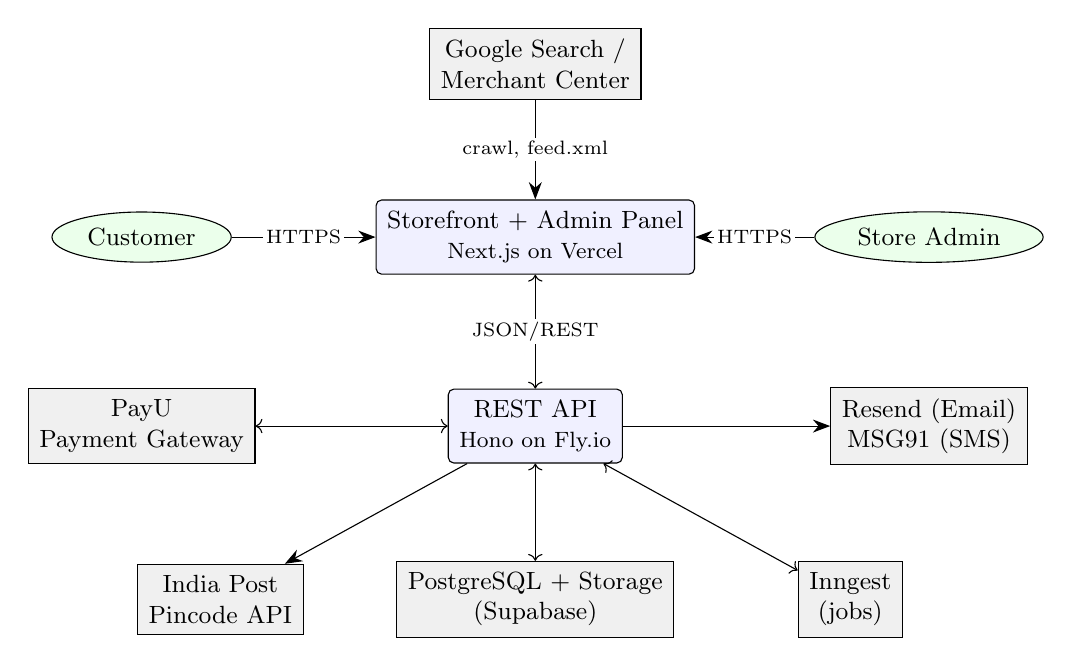
\begin{tikzpicture}[font=\small]
  \node[box] (web) at (0,0) {Storefront + Admin Panel\\\footnotesize Next.js on Vercel};
  \node[box] (api) at (0,-2.4) {REST API\\\footnotesize Hono on Fly.io};
  \node[ext] (db) at (0,-4.6) {PostgreSQL + Storage\\(Supabase)};
  \node[draw,ellipse,fill=green!8] (c) at (-5,0) {Customer};
  \node[draw,ellipse,fill=green!8] (a) at (5,0) {Store Admin};
  \node[ext] (g) at (0,2.2) {Google Search /\\Merchant Center};
  \node[ext] (p) at (-5,-2.4) {PayU\\Payment Gateway};
  \node[ext] (m) at (5,-2.4) {Resend (Email)\\MSG91 (SMS)};
  \node[ext] (pin) at (-4,-4.6) {India Post\\Pincode API};
  \node[ext] (inn) at (4,-4.6) {Inngest\\(jobs)};
  \draw[arr] (c) -- node[lbl]{HTTPS} (web);
  \draw[arr] (a) -- node[lbl]{HTTPS} (web);
  \draw[arr] (g) -- node[lbl]{crawl, feed.xml} (web);
  \draw[arr,<->] (web) -- node[lbl]{JSON/REST} (api);
  \draw[arr,<->] (p) -- (api);
  \draw[arr] (api) -- (m);
  \draw[arr,<->] (api) -- (db);
  \draw[arr] (api) -- (pin);
  \draw[arr,<->] (api) -- (inn);
\end{tikzpicture}
\caption{System context diagram}\label{fig:ctx}
\end{figure}

\subsubsection{Use Case Diagram}
\begin{figure}[H]\centering
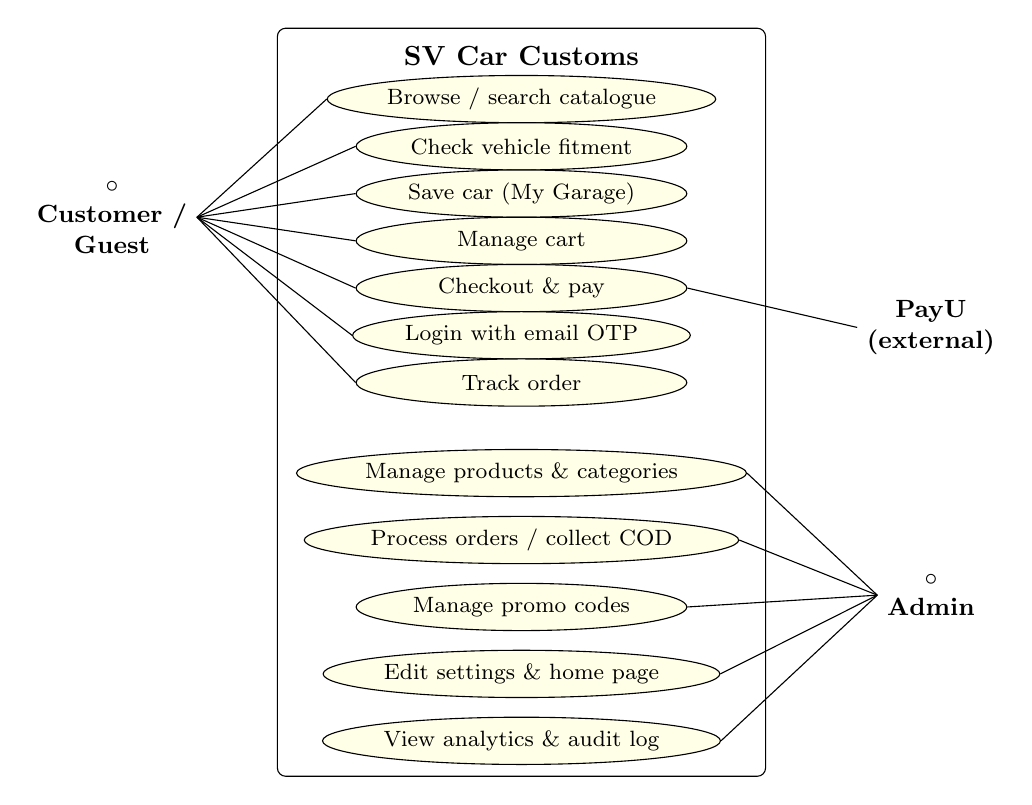
\begin{tikzpicture}
  \draw[rounded corners=3pt] (-3.1,-5.9) rectangle (3.1,3.6);
  \node[font=\bfseries] at (0,3.25) {SV Car Customs};
  \foreach \t [count=\i] in {Browse / search catalogue,Check vehicle fitment,Save car (My Garage),Manage cart,Checkout \& pay,Login with email OTP,Track order}
    \node[uc] (c\i) at (0,3.3-0.6*\i) {\t};
  \foreach \t [count=\i] in {Manage products \& categories,Process orders / collect COD,Manage promo codes,Edit settings \& home page,View analytics \& audit log}
    \node[uc] (a\i) at (0,-1.2-0.85*\i) {\t};
  \node[font=\small\bfseries,align=center] (cust) at (-5.2,1.2) {$\circ$\\Customer /\\Guest};
  \node[font=\small\bfseries,align=center] (adm) at (5.2,-3.6) {$\circ$\\Admin};
  \node[font=\small\bfseries,align=center] (pay) at (5.2,-0.2) {PayU\\(external)};
  \foreach \i in {1,...,7} \draw (cust.east) -- (c\i.west);
  \foreach \i in {1,...,5} \draw (adm.west) -- (a\i.east);
  \draw (pay.west) -- (c5.east);
\end{tikzpicture}
\caption{Use case diagram}\label{fig:uc}
\end{figure}

\subsubsection{Entity-Relationship Diagram}
\begin{figure}[H]\centering
\resizebox{\linewidth}{!}{%
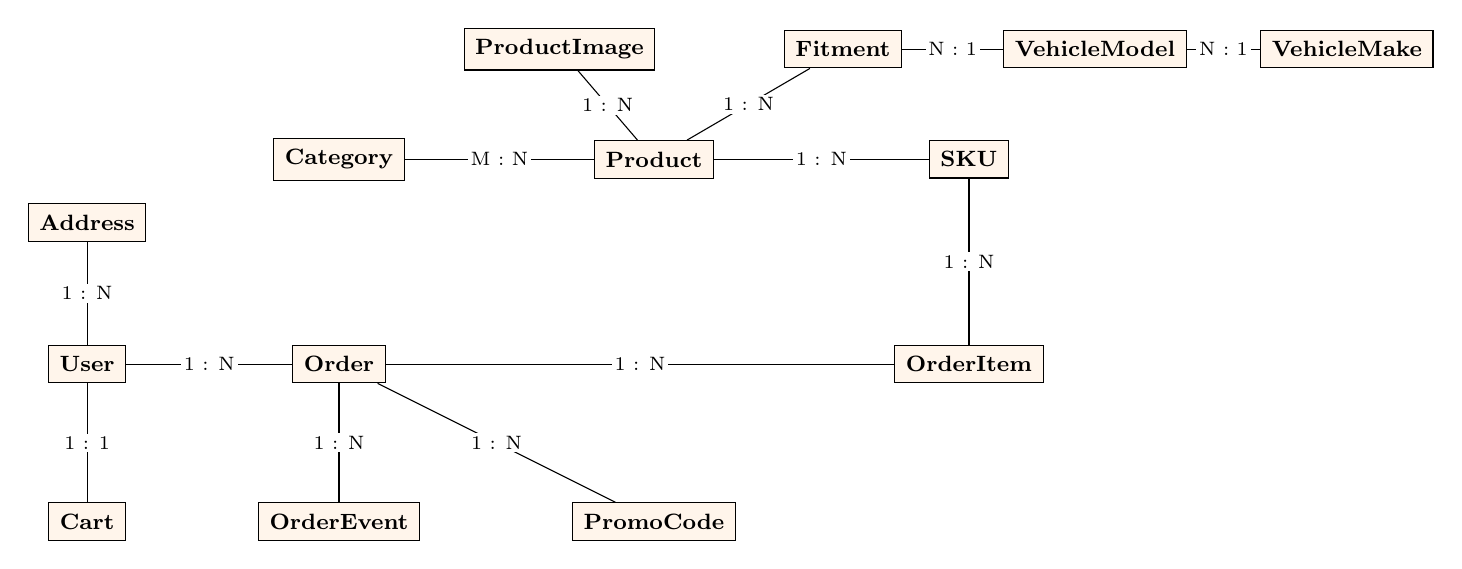
\begin{tikzpicture}[font=\scriptsize]
  \node[ent] (cat) at (-4,2) {Category};
  \node[ent] (prod) at (0,2) {Product};
  \node[ent] (img) at (-1.2,3.4) {ProductImage};
  \node[ent] (sku) at (4,2) {SKU};
  \node[ent] (fit) at (2.4,3.4) {Fitment};
  \node[ent] (vm) at (5.6,3.4) {VehicleModel};
  \node[ent] (vmk) at (8.8,3.4) {VehicleMake};
  \node[ent] (oi) at (4,-0.6) {OrderItem};
  \node[ent] (ord) at (-4,-0.6) {Order};
  \node[ent] (ev) at (-4,-2.6) {OrderEvent};
  \node[ent] (user) at (-7.2,-0.6) {User};
  \node[ent] (addr) at (-7.2,1.2) {Address};
  \node[ent] (cart) at (-7.2,-2.6) {Cart};
  \node[ent] (promo) at (0,-2.6) {PromoCode};
  \draw (cat) -- node[lbl]{M : N} (prod);
  \draw (prod) -- node[lbl]{1 : N} (img);
  \draw (prod) -- node[lbl]{1 : N} (sku);
  \draw (prod) -- node[lbl]{1 : N} (fit);
  \draw (fit) -- node[lbl]{N : 1} (vm);
  \draw (vm) -- node[lbl]{N : 1} (vmk);
  \draw (sku) -- node[lbl]{1 : N} (oi);
  \draw (ord) -- node[lbl]{1 : N} (oi);
  \draw (ord) -- node[lbl]{1 : N} (ev);
  \draw (user) -- node[lbl]{1 : N} (ord);
  \draw (user) -- node[lbl]{1 : N} (addr);
  \draw (user) -- node[lbl]{1 : 1} (cart);
  \draw (promo) -- node[lbl]{1 : N} (ord);
\end{tikzpicture}}
\caption{Simplified entity-relationship diagram (14 of the 28 tables)}\label{fig:er}
\end{figure}

\subsubsection{Data Flow Diagram}
\begin{figure}[H]\centering
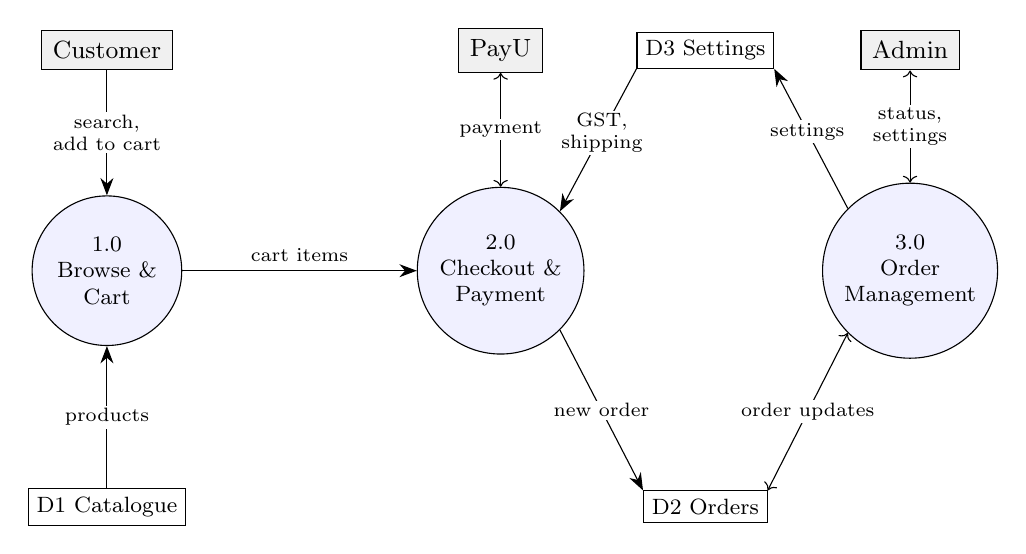
\begin{tikzpicture}[font=\scriptsize]
  \node[ext] (c) at (-5,2.8) {Customer};
  \node[ext] (p) at (0,2.8) {PayU};
  \node[store] (d3) at (2.6,2.8) {D3 Settings};
  \node[ext] (a) at (5.2,2.8) {Admin};
  \node[proc] (p1) at (-5,0) {1.0\\Browse \&\\Cart};
  \node[proc] (p2) at (0,0) {2.0\\Checkout \&\\Payment};
  \node[proc] (p3) at (5.2,0) {3.0\\Order\\Management};
  \node[store] (d1) at (-5,-3) {D1 Catalogue};
  \node[store] (d2) at (2.6,-3) {D2 Orders};
  \draw[arr] (c) -- node[lbl]{search,\\add to cart} (p1);
  \draw[arr] (d1) -- node[lbl]{products} (p1);
  \draw[arr] (p1) -- node[lbl,above=2pt]{cart items} (p2);
  \draw[arr,<->] (p) -- node[lbl]{payment} (p2);
  \draw[arr] (d3.south west) -- node[lbl,pos=0.45]{GST,\\shipping} (p2.north east);
  \draw[arr] (p3.north west) -- node[lbl,pos=0.55]{settings} (d3.south east);
  \draw[arr] (p2.south east) -- node[lbl]{new order} (d2.north west);
  \draw[arr,<->] (d2.north east) -- node[lbl]{order updates} (p3.south west);
  \draw[arr,<->] (a) -- node[lbl]{status,\\settings} (p3);
\end{tikzpicture}
\caption{Level-1 data flow diagram}\label{fig:dfd}
\end{figure}

\subsubsection{Order State Diagram}
\begin{figure}[H]\centering
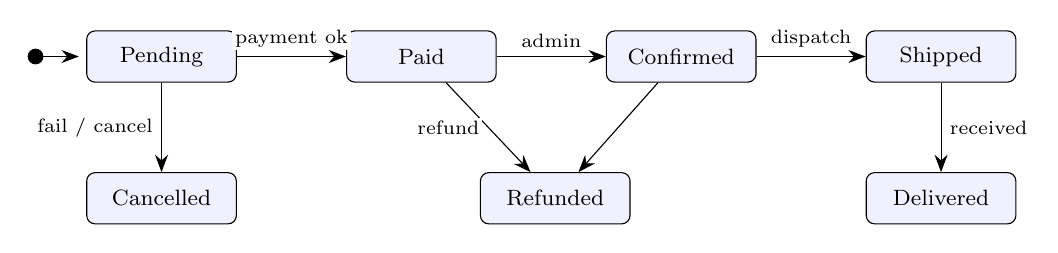
\begin{tikzpicture}[font=\scriptsize]
  \fill (-1.6,0) circle (1mm); \draw[arr] (-1.55,0) -- (-1.05,0);
  \node[state] (pe) at (0,0) {Pending};
  \node[state] (pa) at (3.3,0) {Paid};
  \node[state] (co) at (6.6,0) {Confirmed};
  \node[state] (sh) at (9.9,0) {Shipped};
  \node[state] (ca) at (0,-1.8) {Cancelled};
  \node[state] (re) at (5,-1.8) {Refunded};
  \node[state] (de) at (9.9,-1.8) {Delivered};
  \draw[arr] (pe) -- node[lbl,above=2pt]{payment ok} (pa);
  \draw[arr] (pa) -- node[lbl,above=2pt]{admin} (co);
  \draw[arr] (co) -- node[lbl,above=2pt]{dispatch} (sh);
  \draw[arr] (sh) -- node[lbl,right=2pt]{received} (de);
  \draw[arr] (pe) -- node[lbl,left=2pt]{fail / cancel} (ca);
  \draw[arr] (pa) -- node[lbl,left=2pt]{refund} (re);
  \draw[arr] (co) -- (re);
\end{tikzpicture}
\caption{Order state diagram}\label{fig:state}
\end{figure}

% =====================================================================
\newsection{System Features}
Priority key: \textbf{H} = must have, \textbf{M} = should have, \textbf{L} = nice to have.

\subsection{Description and Priority}
\begin{tabularx}{\linewidth}{@{}l X l@{}}
\toprule
\textbf{Feature} & \textbf{Description} & \textbf{Priority} \\
\midrule
Product Catalogue and Categories & Customers browse products by category. Each product has a title, slug, description, price, compare-at price, images, status (draft / active / archived) and optional variants (SKUs). & High \\
Search and Vehicle Fitment & Customers search by text and find parts that fit their car make and model. & High \\
Cart and Checkout & Customers add items to a cart and check out as a guest or logged-in user. & High \\
Payments & Online payment via PayU, with two methods: full prepaid, or COD where the customer pays a 15\% advance online and the balance on delivery. & High \\
Accounts and Order Tracking & Customers log in with an email OTP and track orders. & Medium \\
Admin Panel & A protected panel for the store owner. & High \\
SEO and Marketing & Make the store discoverable on Google. & Medium \\
\bottomrule
\end{tabularx}

\subsection{Functional Requirements}
\subsubsection{Product Catalogue and Categories}
\begin{reqtable}
FR-CAT-01 & The system shall list all active categories on the home page and in the navigation menu. & H \\
FR-CAT-02 & The system shall show a category page listing its active products with image, name and price, 48 items per page. & H \\
FR-CAT-03 & The system shall show a product detail page with images, price, GST-inclusive note, description, variants and fitment list. & H \\
FR-CAT-04 & A product may belong to more than one category (cross-listing). & M \\
FR-CAT-05 & The PDP shall show related products from the same category. & M \\
FR-CAT-06 & Draft and archived products shall not be visible to customers. & H \\
\end{reqtable}

\subsubsection{Search and Vehicle Fitment}
\begin{reqtable}
FR-SRC-01 & The system shall provide a search box that returns matching active products by name, category and car model. & H \\
FR-SRC-02 & The system shall store vehicle makes and models and link products to them (fitment). & H \\
FR-SRC-03 & The PDP shall list the vehicles a product fits. & M \\
FR-SRC-04 & Search shall return results in under 1 second for the full catalogue. & M \\
FR-SRC-05 & A shopper shall be able to save their car (``My Garage'') and see only the parts that fit it. & M \\
\end{reqtable}

\subsubsection{Cart and Checkout}
\begin{reqtable}
FR-CHK-01 & Users shall add, update quantity and remove items in the cart; the cart persists for logged-in users. & H \\
FR-CHK-02 & Checkout shall collect name, phone, email and shipping address. & H \\
FR-CHK-03 & The system shall validate the 6-digit pincode and auto-fill city and state using the India Post pincode service. & M \\
FR-CHK-04 & The system shall compute subtotal, discount, shipping fee (flat fee, free above an admin-set amount) and GST, and show the total before payment. & H \\
FR-CHK-05 & Guest checkout shall be allowed without creating an account. & H \\
FR-CHK-06 & The system shall create an order with a unique order number before redirecting to payment. & H \\
FR-CHK-07 & Customers shall be able to apply an admin-created promo code (percentage off, optional minimum order, cap, validity window and usage limit). & M \\
\end{reqtable}

\subsubsection{Payments}
\begin{reqtable}
FR-PAY-01 & The system shall redirect the customer to PayU with a signed request (hash) for the payable amount. & H \\
FR-PAY-02 & The system shall verify the PayU response hash and amount on return and on webhook before marking an order paid. & H \\
FR-PAY-03 & For COD, the system shall charge the advance online and record the remaining amount to be collected at delivery. & H \\
FR-PAY-04 & A failed payment shall leave the order pending and allow the customer to retry payment. & H \\
FR-PAY-05 & A background job shall reconcile orders stuck in pending payment with the gateway. & M \\
FR-PAY-06 & The admin shall be able to mark the COD balance as collected. & H \\
\end{reqtable}

\subsubsection{Accounts and Order Tracking}
\begin{reqtable}
FR-ACC-01 & The system shall send a 6-digit OTP to the customer's email and log the user in on correct entry; OTPs expire after 5 minutes, allow 5 attempts and are rate-limited. & H \\
FR-ACC-02 & Users may set a password and log in with it. & L \\
FR-ACC-03 & Logged-in users shall see their order history and saved addresses. & M \\
FR-ACC-04 & Every order shall have a tracking page showing its timeline (placed, paid, confirmed, shipped, out for delivery, delivered). & H \\
FR-ACC-05 & The system shall send email and SMS on order placed, paid and shipped. & M \\
FR-ACC-06 & Guest orders shall be linked to the customer's account when they later sign in with the same email. & L \\
\end{reqtable}

\subsubsection{Admin Panel}
\begin{reqtable}
FR-ADM-01 & Admins shall log in with email and password; all admin routes require a valid admin session. & H \\
FR-ADM-02 & Admins shall create, edit, archive, restore and delete products, including images, variants, fitment and categories. & H \\
FR-ADM-03 & Admins shall preview a draft product through a private, non-indexed preview link before publishing. & M \\
FR-ADM-04 & Admins shall create, edit, archive and reorder categories. & H \\
FR-ADM-05 & Admins shall view, filter and open orders, add timeline events and notes, and update status. & H \\
FR-ADM-06 & Admins shall edit store settings: store name, support phone/email, address, WhatsApp number, GST rate, flat shipping fee and free-shipping threshold. & H \\
FR-ADM-07 & Admins shall edit home-page sections (banners, featured categories and products). & M \\
FR-ADM-08 & Admins shall view WhatsApp and phone leads and newsletter subscribers. & M \\
FR-ADM-09 & Admins shall view sales and visit analytics. & M \\
FR-ADM-10 & Every admin change shall be recorded in an audit log (who, what, when). & M \\
FR-ADM-11 & A change in the admin shall refresh the affected cached storefront pages within one minute. & H \\
FR-ADM-12 & Admins shall create, edit and switch off promo codes. & M \\
\end{reqtable}

\subsubsection{SEO and Marketing}
\begin{reqtable}
FR-SEO-01 & The system shall generate an XML sitemap of all indexable pages and a robots.txt. & H \\
FR-SEO-02 & Every product page shall include Product structured data (JSON-LD) with price, availability and shipping. & H \\
FR-SEO-03 & The system shall publish a Google Merchant Center product feed at /feed.xml. & M \\
FR-SEO-04 & Empty categories and admin/preview pages shall be marked noindex. & M \\
FR-SEO-05 & Users shall be able to subscribe to the newsletter and start a WhatsApp enquiry from the site. & L \\
\end{reqtable}

\subsection{Delivery Status}
All 47 functional requirements are implemented in the submitted code
(\texttt{code/} in the repository) and covered by the automated test suites
(884 passing tests on 26 Nov 2026). The 1-second timing in FR-SRC-04 has not
been measured separately. Non-functional targets that were measured
and not yet met are listed in Section~\ref{sec:nfrstatus}.

% =====================================================================
\newsection{Other Nonfunctional Requirements}
\subsection{Performance Requirements}
\begin{reqtable}
NFR-PER-01 & Catalogue, category and product pages shall be served from cache (static/ISR); a cached page shall respond in under 300\,ms. & H \\
NFR-PER-02 & Largest Contentful Paint shall be under 2.5\,s on a mid-range phone on 4G for the 75th percentile of visits. & M \\
NFR-PER-03 & API responses for cart and checkout shall complete in under 1\,s at normal load. & M \\
NFR-PER-04 & The system shall support at least 200 concurrent shoppers without errors. & M \\
\end{reqtable}

\subsection{Safety and Reliability Requirements}
\begin{reqtable}
NFR-REL-01 & No paid order shall be lost: payment state is confirmed by webhook and by a reconciliation job, independent of the user's browser return. & H \\
NFR-REL-02 & Order data shall be backed up; deleted orders are kept in a backup table. & M \\
NFR-REL-03 & Target availability is 99.5\% per month for the storefront. & M \\
NFR-REL-04 & Errors in production shall be reported to Sentry with request context. & M \\
\end{reqtable}

\subsection{Security Requirements}
\begin{reqtable}
NFR-SEC-01 & All traffic shall use HTTPS. & H \\
NFR-SEC-02 & No card, UPI or bank details shall be stored; payment is handled by PayU. & H \\
NFR-SEC-03 & Admin passwords and OTPs shall be hashed (bcrypt); sessions use signed tokens with expiry. & H \\
NFR-SEC-04 & OTP and login endpoints shall be rate-limited per IP and per email address. & H \\
NFR-SEC-05 & All inputs shall be validated on the server (schema validation) to prevent injection. & H \\
NFR-SEC-06 & Secrets (API keys, gateway salt) shall be kept in environment variables, never in the repository. & H \\
NFR-SEC-07 & Customer personal data shall be used only to fulfil orders, as stated in the Privacy Policy. & H \\
\end{reqtable}

\subsection{Software Quality Attributes}
\begin{itemize}
  \item \textbf{Usability:} mobile-first layout; checkout in at most 3 screens; clear
        price breakdown before payment.
  \item \textbf{Maintainability:} typed code (TypeScript), shared request/response
        contracts between front end and API, modular routes.
  \item \textbf{Testability:} unit and integration tests with Vitest; an end-to-end
        checkout script; tests must pass in CI before deployment.
  \item \textbf{Portability:} API runs in a Docker container and can move to any
        container host.
  \item \textbf{Scalability:} stateless API and cached pages allow horizontal scaling.
\end{itemize}

\subsection{Business Rules}
\begin{itemize}
  \item Displayed prices include GST (default rate 28\%, set in Settings).
  \item Shipping is free above the admin-configured order value (default \rupee5,000);
        below it a flat fee applies (default \rupee200).
  \item COD orders require a 15\% online advance; the balance is collected on delivery.
  \item Only active products can be added to the cart or ordered.
  \item Refunds and returns follow the published Refund Policy.
\end{itemize}

\subsection{Measured Status of Non-functional Targets}\label{sec:nfrstatus}
\begin{tabularx}{\linewidth}{@{}l X l@{}}
\toprule
\textbf{ID} & \textbf{Measurement (26 Nov 2026, live site)} & \textbf{Status} \\
\midrule
NFR-PER-01 & Cached pages answered in 375--437\,ms (median of 3, from India) & Not yet met \\
NFR-PER-02 & Lighthouse mobile lab LCP 9.4--10.8\,s; field data not yet collected & Not yet met \\
NFR-PER-03 & Public API endpoint median 1.26\,s from India & Not yet met \\
NFR-PER-04 & Not load-tested & Not measured \\
NFR-REL-01 & Reconciliation job every 15 minutes; covered by tests & Met \\
NFR-SEC-01--07 & Implemented; covered by unit and route tests & Met \\
\bottomrule
\end{tabularx}

% =====================================================================
\newsection{Other Requirements}
\subsection{External Interface Requirements}
\begin{tabularx}{\linewidth}{@{}l X@{}}
\toprule
\textbf{Interface} & \textbf{Description} \\
\midrule
User interface & Responsive web pages for storefront and admin panel. \\
PayU & HTTPS form post with SHA-512 hash; return URL and server webhook. \\
Resend & REST API for login OTP and transactional email. \\
MSG91 & REST API for order-update SMS. \\
India Post pincode API & Lookup of city/state from pincode (cached 30 days). \\
Supabase & PostgreSQL database and image storage. \\
Inngest & Event-driven and scheduled background jobs. \\
Google & Sitemap, structured data and /feed.xml for Merchant Center. \\
\bottomrule
\end{tabularx}

\subsection{Legal and Regulatory}
The store shall publish Terms, Privacy, Refund and Shipping policies and comply with
the Indian IT Act and the Consumer Protection (E-Commerce) Rules, 2020 (seller name,
address, grievance contact and return policy shown on the site).

\subsection{Future Enhancements}
\begin{itemize}
  \item Verified-purchase customer reviews and ratings.
  \item Automatic courier booking and live shipment tracking.
  \item Native Android app.
\end{itemize}

\end{document}
